\documentclass[10pt,a4paper]{article}
\usepackage[margin=18mm]{geometry}
\usepackage[T1]{fontenc}
\usepackage{lmodern}
\usepackage{amsmath,amssymb,mathtools}
\usepackage{microtype}
\usepackage{graphicx}
\usepackage[hidelinks]{hyperref}
\setlength{\parindent}{0pt}
\setlength{\parskip}{4pt}
\setlength{\abovedisplayskip}{5pt}
\setlength{\belowdisplayskip}{5pt}
\newcommand{\R}{\mathbb R}
\newcommand{\E}{\mathbb E}
\newcommand{\ip}[2]{\langle #1,#2\rangle}
\newcommand{\norm}[1]{\left\|#1\right\|}
\DeclareMathOperator{\dist}{dist}
\hypersetup{pdftitle={Stochastic FRAMES: nonconvex row-sampled least squares},
 pdfsubject={Problem, initialization, parameters, gaps, feasibility, and plots}}

\begin{document}
\begin{center}
{\Large\bfseries Stochastic FRAMES: experiment specification}\\[3pt]
{\large Nonconvex $\ell_1$-constrained least squares in dimension $1024$}\\[2pt]
14 October 2026 \quad $\cdot$ \quad Uniform sampling of individual data rows
\end{center}

\textbf{Problem.} With $d=m=1024$, the problem and its four ingredients are
\[
\boxed{\min_{x\in C} f(x)+g(Tx),\qquad
 f(x)=\norm{Ax-B}_2^2-\frac58(u^\top x)^2,}
\]
\[
C=\{x\in\R^{1024}:\norm{x}_1\le1\},\qquad T=I_{1024},\qquad
g(z)=\iota_D(z)=\begin{cases}0,&z\in D,\\+\infty,&z\notin D,\end{cases}
\quad D=\R_+^{1024}.
\]
Thus original feasibility means $x\ge0$ and $\sum_jx_j\le1$.
The vectors $a,u\in\R^{1024}$ are
\[
a_j=\begin{cases}
1/32,&1\le j\le64,\\
-3/128,&65\le j\le128,\\
1/128,&129\le j\le1024,
\end{cases}
\qquad
u_j=\begin{cases}
(-1)^{j-1}/8,&1\le j\le64,\\
0,&65\le j\le1024.
\end{cases}
\]
Define a Hadamard matrix recursively and set the data matrix and response to
\[
\mathsf W_1=[1],\qquad
\mathsf W_{2n}=\begin{pmatrix}\mathsf W_n&\mathsf W_n\\
\mathsf W_n&-\mathsf W_n\end{pmatrix},\qquad
\boxed{A=\frac{\mathsf W_{1024}\operatorname{diag}(c)}{\sqrt{2048}},\qquad B=Aa.}
\]
The signs $c_j\in\{-1,1\}$ are drawn independently and uniformly once, using
NumPy's default random generator with seed $20261014$, and fixed for every run.
Since $A^\top A=I/2$, the least-squares term is $\norm{x-a}_2^2/2$.
Writing $Q=I-\frac54uu^\top$, we have
\[
\nabla f(x)=Qx-a,\qquad
\nabla^2 f=Q,\qquad
\operatorname{spec}(Q)=\{-1/4,1\}.
\]
The shared concave quadratic makes $f$ nonconvex; its gradient is globally
$1$-Lipschitz.

\textbf{Row-sampled stochastic gradient.} Let $A_i$ be row $i$ of $A$, and $B_i$
the corresponding response. The finite sum and sampled gradient are
\[
f=\frac1m\sum_{i=1}^m f_i,\qquad
f_i(x)=m(A_ix-B_i)^2-\frac58(u^\top x)^2,
\]
\[
\boxed{q_k=2m(A_{i_k}x_k-B_{i_k})A_{i_k}^\top
       -\frac54(u^\top x_k)u,\qquad
 i_k\sim\operatorname{Uniform}\{1,\ldots,m\}.}
\]
Rows are sampled independently with replacement; the concave term is evaluated
exactly. If $\mathcal F_k$ denotes the history before the fresh row draw, then
\[
\E[q_k\mid\mathcal F_k]=\nabla f(x_k),\qquad
\E[\norm{q_k-\nabla f(x_k)}_2^2\mid\mathcal F_k]
=1023\norm{x_k-a}_2^2\le\frac{318153}{256}.
\]

\textbf{Initialization and parameters.} For each seed $s\in\{0,\ldots,7\}$, draw
$J_s$ uniformly from $\{1,\ldots,1024\}$ independently of all row draws, and set
\[
\boxed{x_0^{(s)}=-e_{J_s}.}
\]
Here $e_j$ has entry $1$ in position $j$ and zeros elsewhere. Thus the initial point
has one random entry equal to $-1$, with $\norm{x_0^{(s)}}_1=1$ and
$\dist_D(x_0^{(s)})=1$. Initialize momentum with the first sampled gradient.
Use $N=32768$ updates per seed, $8$ seeds, float64 arithmetic, and
\[
\boxed{\gamma_k=(k+1)^{-3/4},\qquad
\beta_k=(k+1)^{-1/4},\qquad
\alpha_k=(k+1)^{-1/2},\qquad 0\le k<N.}
\]
These are respectively the Frank--Wolfe step size, smoothing parameter, and weight
on the new stochastic gradient. All prefactors are $1$; one row is sampled per update.

\newpage
\textbf{Gap and feasibility notation.} Define $(x_k)_-=\min(x_k,0)$ coordinatewise,
and set
\[
z_k:=\nabla f(x_k)=Qx_k-a,\qquad h_k:=z_k+\frac{(x_k)_-}{\beta_k}.
\]
The reported gaps use these exact vectors, rather than the sampled gradient:
\begin{align*}
G_k
&:=\max_{v\in C}\ip{h_k}{x_k-v}
 =\boxed{\ip{h_k}{x_k}+\norm{h_k}_\infty},
&&\text{smoothed Frank--Wolfe gap},\\[3pt]
H_k
&:=\max_{v\in C\cap D}\ip{z_k}{x_k-v}
 =\boxed{\ip{z_k}{x_k}+\max\{0,-\min_jz_{k,j}\}},
&&\text{original constrained gap},\\[3pt]
\delta_k
&:=\dist_D(x_k)
 =\boxed{\norm{(x_k)_-}_2},
&&\text{feasibility violation}.
\end{align*}
Since $x_k\in C$, $G_k\ge0$. However, $H_k$ can be negative when $x_k\notin D$;
the cumulative original-gap plot therefore reports $|H_k|$. Feasibility and the
original gap are interpreted together.

\textbf{What the plots average.} For $Z_k\in\{G_k,|H_k|,\delta_k\}$, define
\[
\overline Z_N^{(s)}=\frac1N\sum_{k=0}^{N-1}Z_k^{(s)},\qquad
\widehat A_Z(N)=\frac18\sum_{s=0}^{7}\overline Z_N^{(s)}.
\]
Every pre-update iterate $x_0,\ldots,x_{N-1}$ is included. Thin curves are individual
seed averages; the black curve is $\widehat A_Z(N)$; the band is $\pm2$ standard errors
across the eight seed averages (descriptive). The dashed $N^{-1/3}$ line is a comparison
slope only, not a claimed convergence guarantee or a numerical upper bound.

\medskip
\textbf{Plots.} Eight seeds with random negative-vertex initialization.
\begin{center}
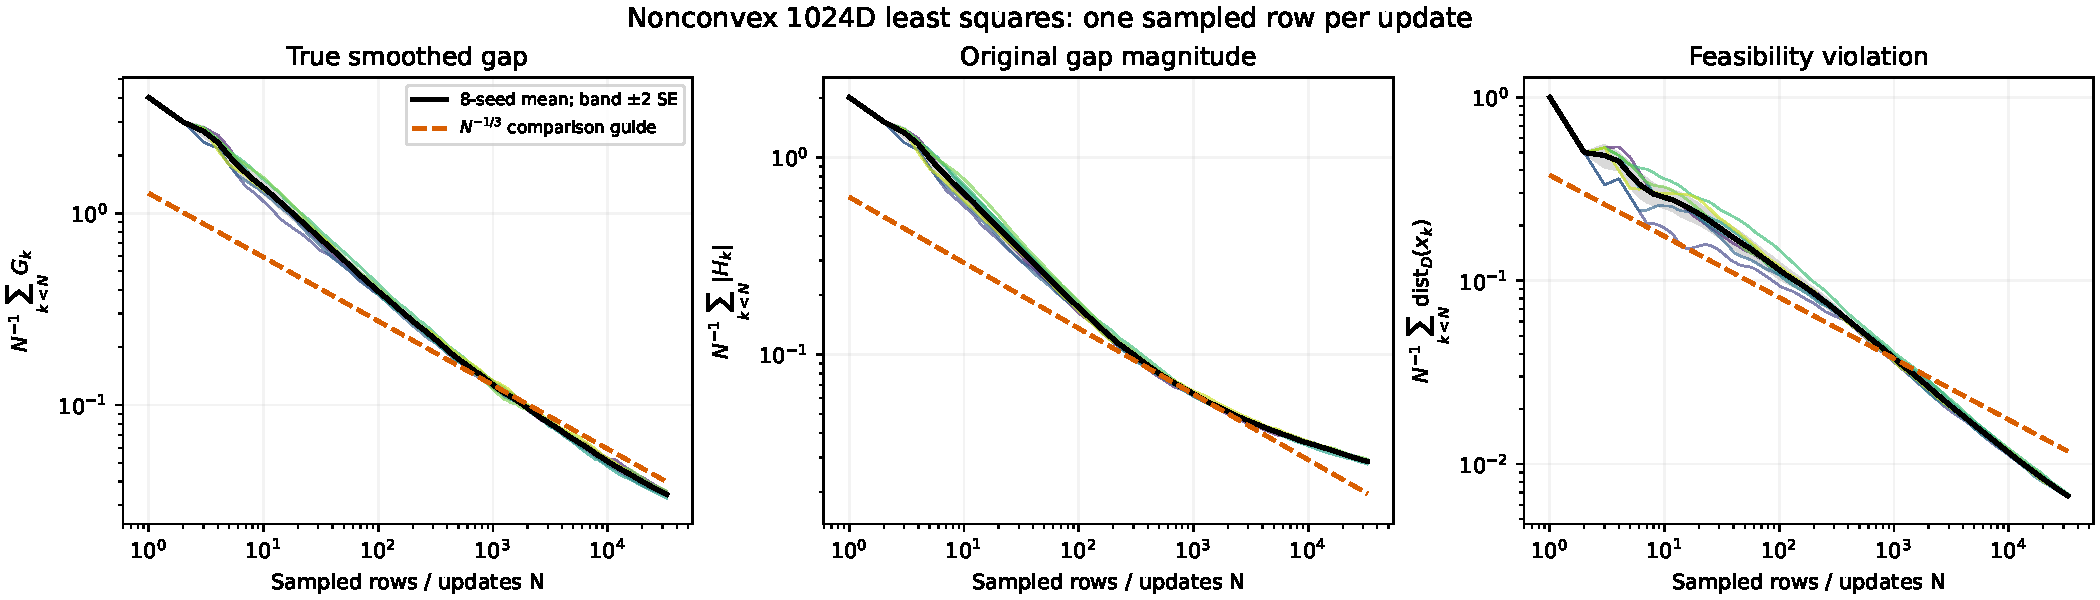
\includegraphics[width=\linewidth]{gaps_feasibility.pdf}
\end{center}
{\small Cumulative averages of $G_k$, $|H_k|$, and $\delta_k$ over all recorded iterates.}

\medskip
\begin{center}
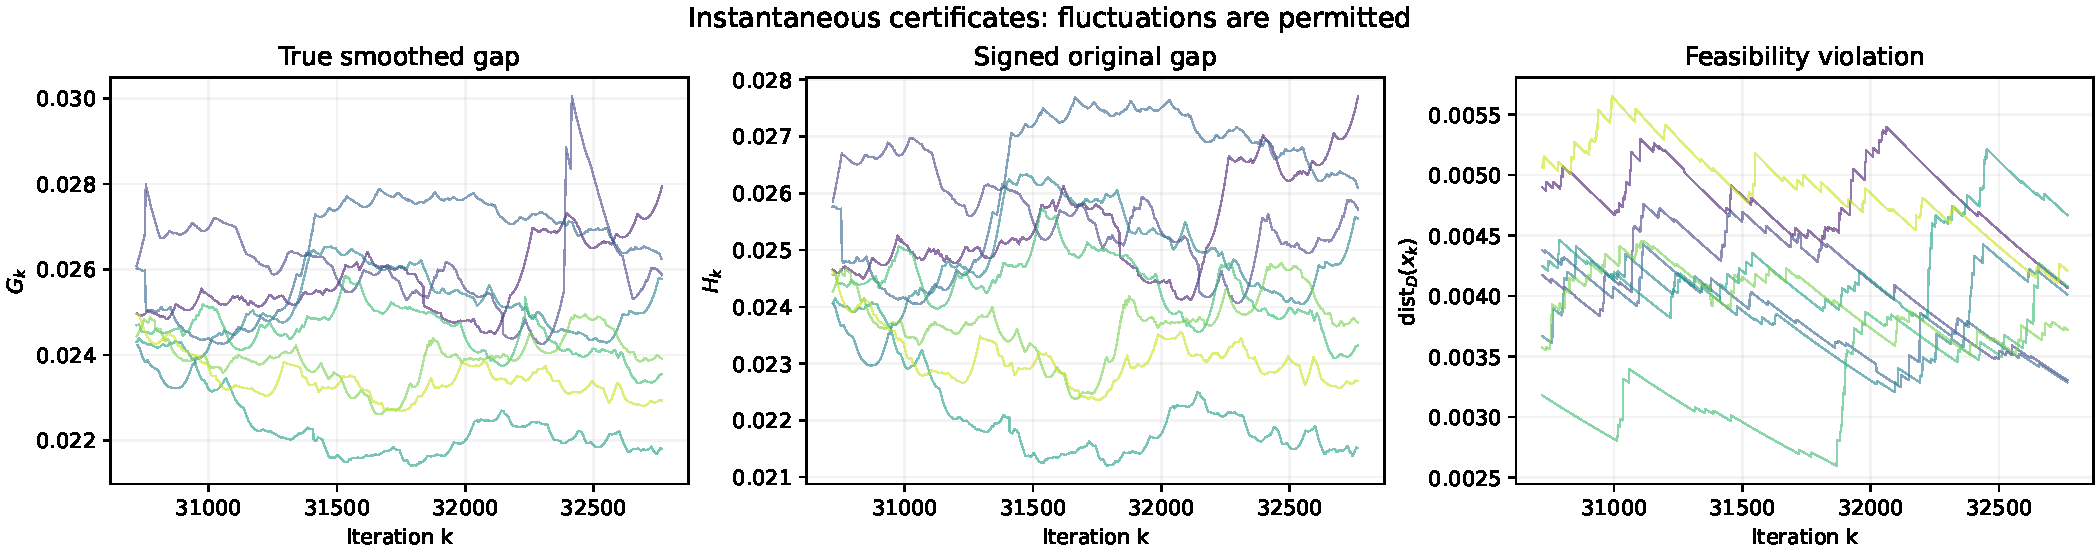
\includegraphics[width=\linewidth]{instantaneous_certificates.pdf}
\end{center}
{\small Individual values of $G_k$, signed $H_k$, and $\delta_k$ during the final $2048$
iterations. Each color represents one seed.}
\end{document}
